\begin{frame}
\frametitle{Dicas}
\framesubtitle{}
\centering
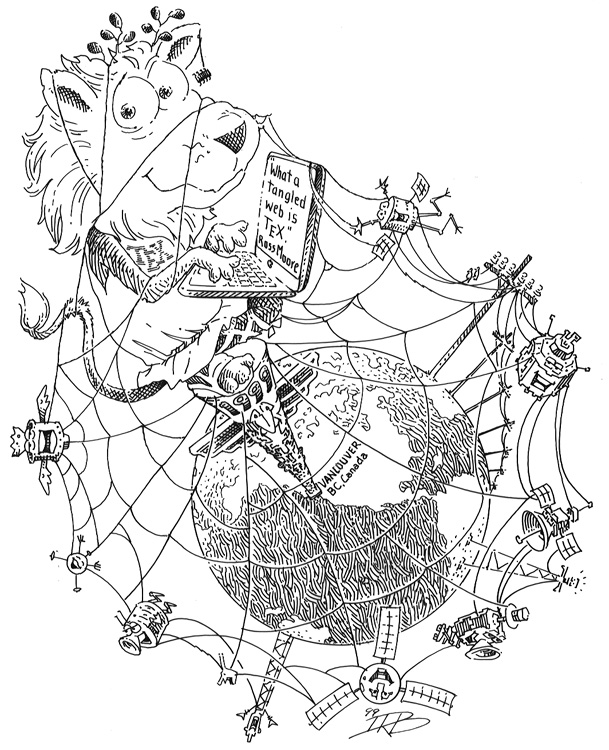
\includegraphics[width=0.4\linewidth]{figures/lion05.png}
\end{frame}

\begin{frame}[fragile]
\frametitle{Controle de versão e colaboração}
\framesubtitle{}
\begin{itemize}
\item Git, Mercurial, Subversion, CVS, etc
\item servidor remoto ou local
\item Overleaf
\end{itemize}
\end{frame}

\begin{frame}
\frametitle{Dicas}
\framesubtitle{Algumas dicas para facilitar}
  \begin{itemize}
  \item google it
  \item \hrefcolor{https://www.doi2bib.org/}{doi2bib}, \hrefcolor{https://books.google.com}{Google Books},
	  \hrefcolor{https://www.xarg.org/tools/isbn-to-bibtex/}{isbn2bib},
	  \hrefcolor{https://www.ottobib.com/}{isbn2bib} % {\sout{isbn2bib}},
	  \hrefcolor{https://manas.tungare.name/software/isbn-to-bibtex}{isbn2bib},
	  \hrefcolor{https://arxiv2bibtex.org/}{arxiv2bibtex}
  \item \hrefcolor{https://www.tablesgenerator.com/}{tables generator}, \hrefcolor{https://www.latex-tables.com/}{latex tables}
  \item \hrefcolor{https://pandoc.org/}{pandoc}, \hrefcolor{https://www.ctan.org/pkg/markdown}{markdown package}
  \item \hrefcolor{http://detexify.kirelabs.org/classify.html}{detexify}
  \item \hrefcolor{https://quicklatex.com/}{quick latex - render png}
  \item \hrefcolor{http://texample.net/}{texample}, \hrefcolor{https://texblog.org/}{texblog}
  \item \hrefcolor{http://www.wolframalpha.com/input/?i=int+sin{x^2}\%2Bsqrt{x}+dx}{TeX notation and Wolfram Alpha computation}
  \end{itemize}
\end{frame}


\begin{frame}[fragile]
\frametitle{Ajuda}
\framesubtitle{Onde buscar ajuda?}
  \begin{description}
  \item[lshort] : \hrefcolor{http://www.ctan.org/tex-archive/info/lshort/portuguese/ptlshort.pdf}{Introdução ao \LaTeX}
  \item[livro \LaTeX{}] : \hrefcolor{http://www.vivas.eng.br/index.php/latex-elaboracao-de-documentos-digitais/}{\LaTeX{}: elaboração de documentos digitais}
  \item[wikibooks] : \hrefcolor{http://en.wikibooks.org/wiki/LaTeX}{http://en.wikibooks.org/wiki/LaTeX}
  \item[CTAN] : \hrefcolor{http://www.ctan.org/}{http://www.ctan.org/}
  \begin{enumerate}
  \item \hrefcolor{https://ctan.org/pkg/fancyhdr}{Fancyheadings package}
  \item \hrefcolor{https://ctan.org/pkg/beamer}{Beamer package} (apresentações)
  \item \hrefcolor{https://ctan.org/pkg/geometry}{Geometry package}
  \item \hrefcolor{https://ctan.org/pkg/hyperref}{Hyperref package}
  \item \hrefcolor{http://en.wikibooks.org/wiki/LaTeX/Packages}{Packages list}
  \end{enumerate}
  \item[google group] : \hrefcolor{https://groups.google.com/forum/?hl=en\#!forum/comp.text.tex}{comp.text.tex}
  \item[latex forum] : \hrefcolor{https://latex.org/forum/}{latex.org/forum/}
  \item[Overleaf] : \hrefcolor{https://www.overleaf.com/learn}{Overleaf - learn}
  \item[StackExchange] : \hrefcolor{https://tex.stackexchange.com/}{StackExchange} 
  \item[tutorial] : \hrefcolor{https://www.latex-tutorial.com/}{\LaTeX{} Tutorial}
  \end{description}
\end{frame}
